\documentclass[letter, 11pt]{article}
%% ================================
%% Packages =======================
\usepackage[utf8]{inputenc}      %%
\usepackage[T1]{fontenc}         %%
\usepackage{lmodern}             %%
\usepackage[spanish]{babel}      %%
\decimalpoint                    %%
\usepackage{fullpage}            %%
\usepackage{fancyhdr}            %%
\usepackage{float}               %%
\usepackage{graphicx}            %%
\usepackage{amsmath}             %%
\usepackage{amssymb}             %%
\usepackage{color}               %%
\usepackage{mdframed}            %%
\usepackage[colorlinks]{hyperref}%%
%% ================================
%% ================================

%% ================================
%% Page size/borders config =======
\setlength{\oddsidemargin}{0in}  %%
\setlength{\evensidemargin}{0in} %%
\setlength{\marginparwidth}{0in} %%
\setlength{\marginparsep}{0in}   %%
\setlength{\voffset}{-0.5in}     %%
\setlength{\hoffset}{0in}        %%
\setlength{\topmargin}{0in}      %%
\setlength{\headheight}{54pt}    %%
\setlength{\headsep}{1em}        %%
\setlength{\textheight}{8.5in}   %%
\setlength{\footskip}{0.5in}     %%
%% ================================
%% ================================

%% =============================================================
%% Headers setup, environments, colors, etc.
%%
%% Header ------------------------------------------------------
\fancypagestyle{firstpage}
{
  \fancyhf{}
  \lhead{
\includegraphics[height=4.5em]{LogoDFI.jpg}}
  \rhead{FI3104-1 \semestre\\
         Métodos Numéricos para la Ciencia e Ingeniería}
  \fancyfoot[C]{\thepage}
}

\pagestyle{plain}
\fancyhf{}
\fancyfoot[C]{\thepage}
%% -------------------------------------------------------------
%% Environments -------------------------------------------------
\newmdenv[
  linecolor=gray,
  fontcolor=gray,
  linewidth=0.2em,
  topline=false,
  bottomline=false,
  rightline=false,
  skipabove=\topsep
  skipbelow=\topsep,
]{ayuda}
%% -------------------------------------------------------------
%% Colors ------------------------------------------------------
\definecolor{gray}{rgb}{0.5, 0.5, 0.5}
%% -------------------------------------------------------------
%% Aliases ------------------------------------------------------
\newcommand{\scipy}{\texttt{scipy}}
%% -------------------------------------------------------------
%% =============================================================

%% =============================================================================
%% CONFIGURACION DEL DOCUMENTO =================================================
%% Llenar con la información pertinente al curso y la tarea
%%
\newcommand{\fechaentrega}{15/09/2019 23:59 hrs}
\newcommand{\semestre}{2019B}
%% =============================================================================
%% =============================================================================


\begin{document}
\thispagestyle{firstpage}

\begin{center}
  {\uppercase{\LARGE \bf Informe Tarea 5}}
\end{center}

\noindent{\Large Tomás Rojas C.}\\
\noindent{\Large RUT:19.688.339-8}\\
\noindent{\Large Github: @tomasrojasc}


%% =============================================================================
%% =============================================================================









\section{Problema.}

Primero, vamos a manipular la ecuación entregada en el enunciado para dejarla como un sistema de ecuaciones diferenciales de primer orden.

\begin{align*}
  \dot{\Omega}&=-\frac{g}{L}[1+8\lambda^2\cos(\omega_1 t)]\sin\phi\\
  \dot{\phi}&=\Omega
\end{align*}

con las condiciones iniciales:


\begin{align*}
  \Omega(0)&=0\\
  \phi(0)&=\phi_0
\end{align*}


\section{Implementación.}

A continuación se implementó el método Runge-Kutta 4 para un sistema de dos ecuaciones diferenciales lineales ordinarias. Los parámetros a variar entre las seis veces que se ejecutó el programa son: $\lambda$ y $\phi_0$. Para resolver este problema se implementó RK4 pensando en que las dos ecuaciones mostradas pueden ser representadas por dos funciones que, después de usar datos del enunciado, quedan de la siguiente manera:

\begin{align*}
  f_1(t, \Omega, \phi, g, \lambda)&=\dot{\Omega}=-\frac{g}{L}[1+8\lambda^2\cos(4\lambda \sqrt{g} t)]\sin\phi\\
  f_2(t, \Omega, \phi)&=\dot{\phi}=\Omega
\end{align*}


Pese a que ambas funciones no dependen de todos
los argumentos entre paréntesis, es más fácil
escribirlas así al momento de implementar el
algoritmo, ya que hace que el código sea
visualmente más entendible, por lo que nos
vamos a apegar a esa notación pese a que en
estricto rigor no es correcta.

Con las funciones que describen las EDOs,
podemos implementar RK4 sin problemas en un
forloop.

\section{Resultados.}

En primer lugar vamos a fijar $g=10$ como
aproximación para la aceleración de gravedad en
la superficie terrestre, pero el parámetro
puede cambiarse para ver qué pasaría en la
superficie de algún otro planeta o en alguna
otra situación, además vamos a fijar el paso en
el tiempo como $h=0.001$ ya que se observó que
es un buen número tanto por tema de tiempo como
por que la función de movimiento queda
suficientemente suave como para ser graficada.
En cualquier caso, no se recomienda correr
todos los casos de una sola vez.

En esta sección se van a presentar, para cada
caso un gráfico del recorrido que hizo la masa
en el péndulo y para los casos más
interesantes, también se presentará el espacio
de fase asumiendo la masa $m=1$ por simplicidad.


\subsection{Primeros casos: $\phi_0=0.00339$.}

\begin{figure*}[h!]
 \centering
 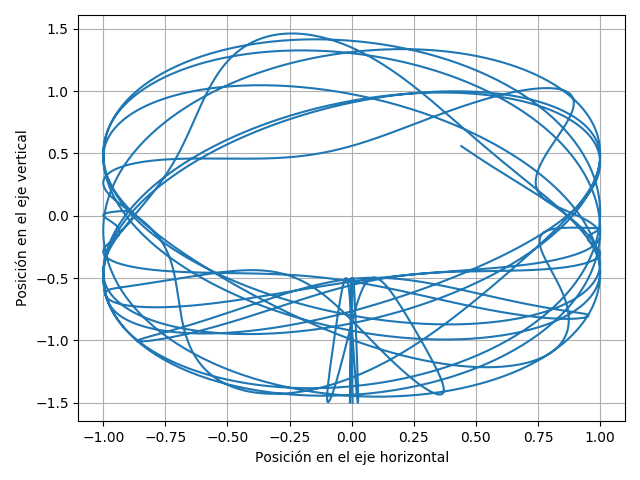
\includegraphics[width=0.5\textwidth]{./imagenes/img1.png}
 \caption{Camino recorrido con $\lambda = 1$.}
\end{figure*}

\begin{figure*}[h!]
 \centering
 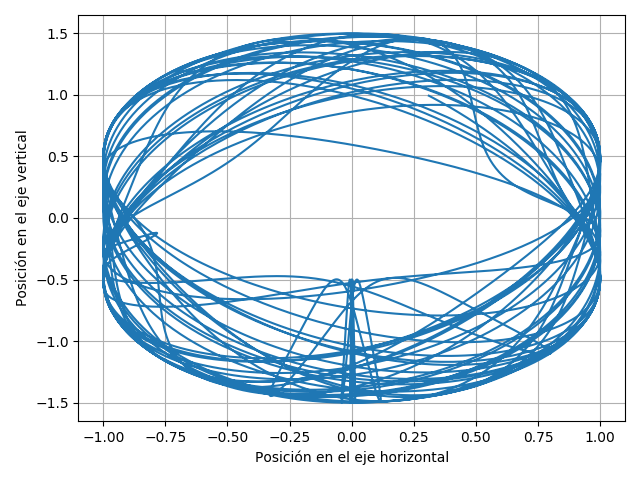
\includegraphics[width=0.5\textwidth]{./imagenes/img2.png}
 \caption{Camino recorrido con $\lambda = 2$.}
\end{figure*}

\begin{figure*}[h!]
 \centering
 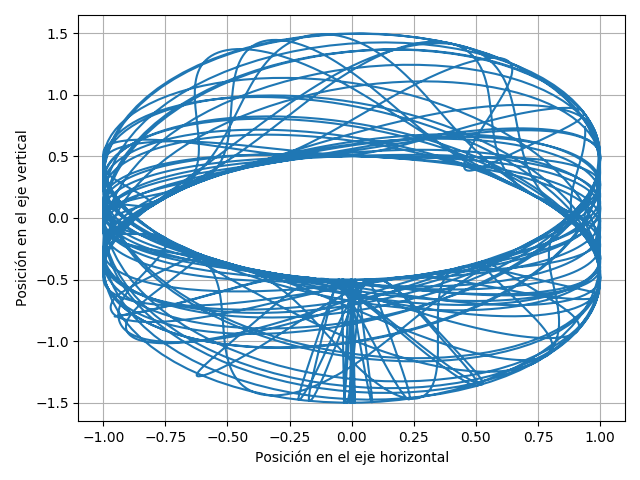
\includegraphics[width=0.5\textwidth]{./imagenes/img3.png}
 \caption{Camino recorrido con $\lambda = 3$.}
\end{figure*}



\newpage


\subsection{Segundos casos: $\phi_0 = \pi - 0.00339$.}

\begin{figure*}[h!]
 \centering
 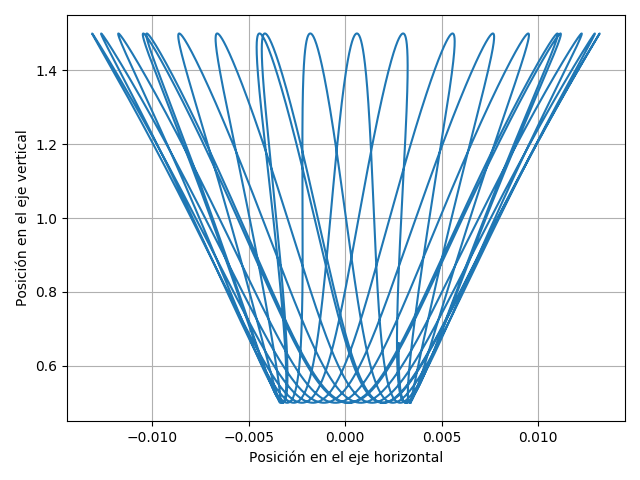
\includegraphics[width=0.5\textwidth]{./imagenes/img4.png}
 \caption{Camino recorrido con $\lambda = 1$.}
\end{figure*}

\begin{figure*}[h!]
 \centering
 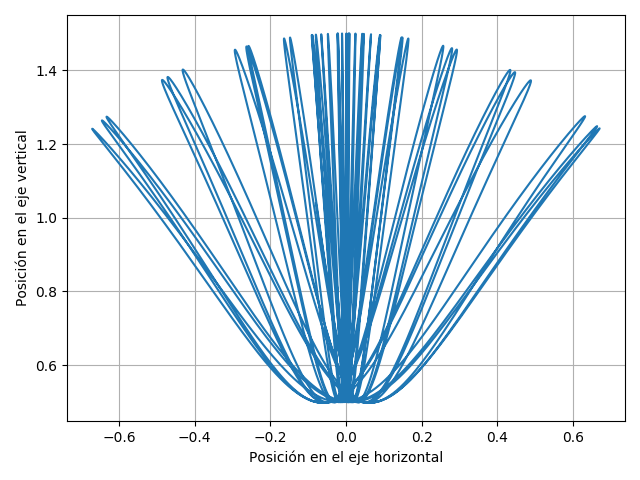
\includegraphics[width=0.5\textwidth]{./imagenes/img5.png}
 \caption{Camino recorrido con $\lambda = 2$.}
\end{figure*}

\begin{figure*}[h!]
 \centering
 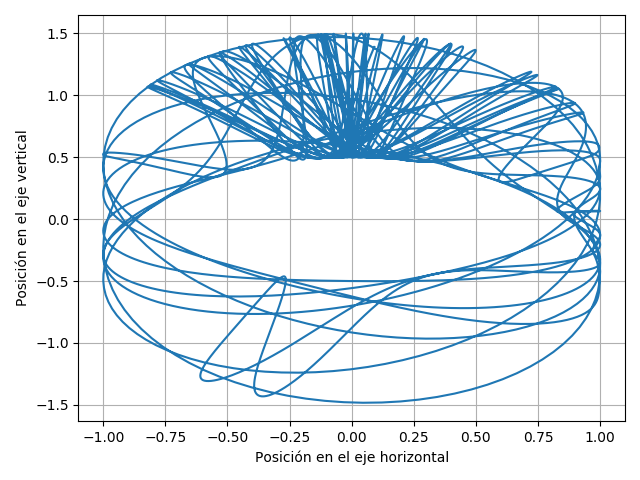
\includegraphics[width=0.5\textwidth]{./imagenes/img6.png}
 \caption{Camino recorrido con $\lambda = 3$.}
\end{figure*}

\newpage

\subsection{Análisis}
Vemos que tenemos un sistema cuyos puntos de equilibrio claramente son cuando nuestra masa parte en una posición vertical, para notar esto, veamos los espacios de fase con $\lambda=1$, tanto partiendo con la masa en alto, o desde abajo.


\begin{figure*}[h!]
 \centering
 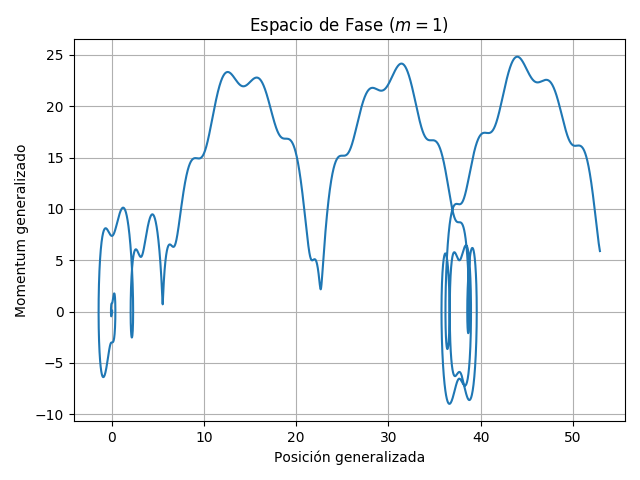
\includegraphics[width=0.7\textwidth]{./imagenes/img1_phase.png}
 \caption{Espacio de fase con:  $\phi_0=0.00339; \quad \lambda = 1$.}
\end{figure*}



\begin{figure*}[h!]
 \centering
 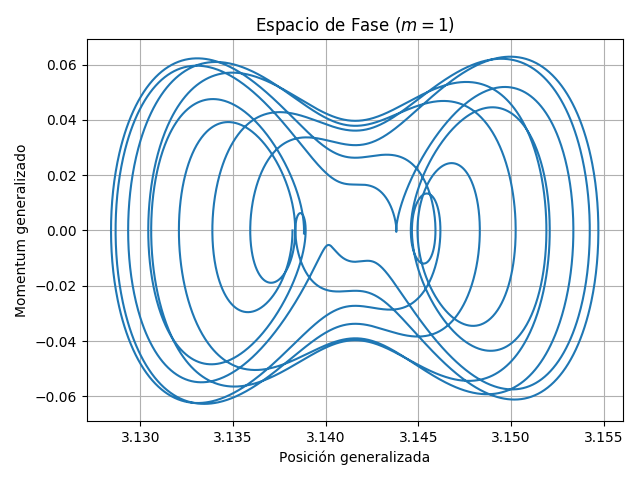
\includegraphics[width=0.7\textwidth]{./imagenes/img4_phase.png}
 \caption{Espacio de fase con:  $\phi_0=\pi-0.00339; \quad \lambda = 1$.}
\end{figure*}


Notemos que para el caso que parte con $\phi_0=\pi-0.00339$ tenemos un equilibrio estable, que notamos con un movimiento en el espacio de fase muy acotado, característico de este tipo de equilibrios, mientras que en la figura 7 vemos cómo pese a que se iba a quedar en un espacio acotado, se fue del equilibrio, comportamiento característico de los equilibrios inestables. este comportamiento se puede corroborar mirando la figura 1 que es el recorrido de este mismo caso.



\newpage

\newpage

\section{Desempeño.}




La implementación de RK4 desarrollada en el código se demoró en promedio $\approx 0.451 [s]$, por lo que, teniendo en cuenta que el largo de los arreglos utilizados es de 10000 datos, no está tan mal.

Por otro lado, la librería scipy tiene un módulo dedicado a la ingtegración numérica en scipy.integrate, el solver que se usó es scipy.integrate.solve\_ivp con el método RK45 del mismo módulo de la librería. Al ejecutar este método, vemos que en promedio se demoró en promedio $\approx 1.654$ lo cual a primera vista es bastante sorprendente, pero hay que tener en cuenta que nuestra implementación es mucho más específica que la que trae la librería scipy, partiendo por que esta clase en particular tiene muchas opciones, si nos ponemos a ver la clase, vemos que tiene muchas operaciones condicionales anidadas por lo que eso compromete su eficiencia. Por otro lado nuestra clase Setup existe sabiendo de antemano lo que se le va a ingresar y qué tipo de funciones entran, por ejemplo, la función sabe que es un sistema de dos ecuaciones diferenciales, y se implementa RK4 sin llamar a ningún módulo externo, entre otros detalles que mejoran el desempeño en este caso particular.
Otra cosa es que quizá nuestra implementación gana en cortas distancias pero pierde en largas, es decir, quizá el número de puntos a evaluar no es suficiente para explotar la eficiencia de la implementación del módulo scipy.


\section{Conclusión.}

Vemos que pese a que existen librerías en donde se implementan muchas cosas para la resolución de problemas numéricos, pueden haber casos en que sí valga la pena implementar algo, siempre que el tiempo y las características del problema permitan una implementación que proporcione mejoras dignas de ser consideradas. En este caso, el tiempo invertido en la implementación, no vale los pocos segundos de cómputo ganados, aunque sí nos da una visión mucho mejor de cómo funcionan estos algoritmos y cómo usarlos.









\end{document}
